% !TeX document-id = {fc374fa5-1b07-442b-a1fa-fa8a2a7461e5}
% !TeX TXS-program:compile = txs:///pdflatex/[--shell-escape]
\documentclass[export,border=0pt]{standalone}
\usepackage{tikz,filecontents, pgfplots}
\usepackage{pgf}
\usepackage{pgfplotstable}
\pgfplotsset{compat=1.3}
\usepackage{amsmath,bm}
\usetikzlibrary{arrows,
	arrows.meta,
	decorations.pathmorphing,
	calc,%
	decorations.pathmorphing,%
	decorations.markings,
	fadings,%
	shadings,%
	positioning,
	spy,
	shapes,
	shapes.geometric,
	shapes.arrows,
	fit,
	plotmarks,}
\usepackage{animate}
\usepackage{newtxtext}
\usepackage{newtxmath}
\begin{document}
\begin{animateinline}[loop]{10}
\multiframe{6}{i=1+1}{	
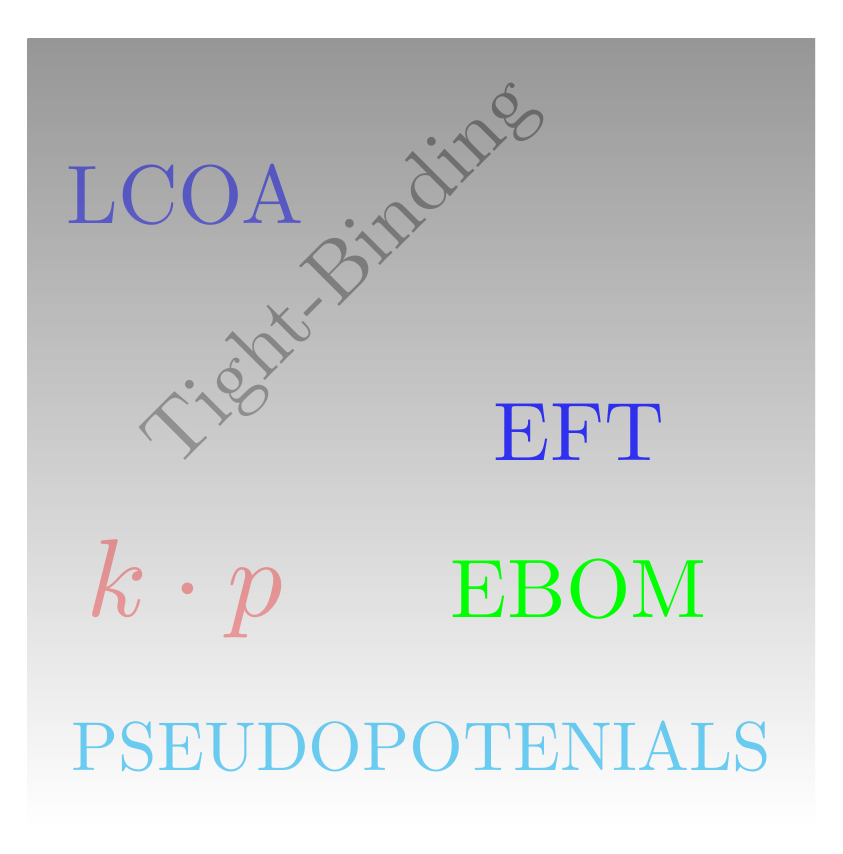
\begin{tikzpicture}
\foreach [count=\xi from 1]\x in {1,...,\i}{
	\pgfmathparse{int(\x)}

	\ifnum\pgfmathresult=1
			\shade[ color=blue, opacity=0.25] (0,0)--(0,10)--(10,10)--(10,0)--cycle;
			\node[scale=3,rotate=45] at (4,7) {Tight-Binding};
	\fi
	\ifnum\pgfmathresult=2
	\shade[  color=green, opacity=0.25] (0,0)--(0,10)--(10,10)--(10,0)--cycle;
	\node[scale=4,red] at (2,3) {$k\cdot p$};
	\fi
		\ifnum\pgfmathresult=3
	\shade[ color=magenta, opacity=0.25] (0,0)--(0,10)--(10,10)--(10,0)--cycle;
	\node[scale=3,blue] at (2,8) {LCOA};
	\fi
		\ifnum\pgfmathresult=4
	\shade[ color=orange, opacity=0.25] (0,0)--(0,10)--(10,10)--(10,0)--cycle;
	\node[scale=2.5,cyan] at (5,1) {PSEUDOPOTENIALS};
	\fi
		\ifnum\pgfmathresult=5
	\shade[  color=red, opacity=0.25] (0,0)--(0,10)--(10,10)--(10,0)--cycle;
	\node[scale=3,blue] at (7,5) {EFT};
	\fi
	
		\ifnum\pgfmathresult=6
	\shade[  color=cyan, opacity=0.25] (0,0)--(0,10)--(10,10)--(10,0)--cycle;
	\node[scale=3,green] at (7,3) {EBOM};
	\fi
	
}
\end{tikzpicture}}
\end{animateinline}
\end{document}